
% This is a Basic Assignment Paper but with like Code and stuff allowed in it. 

\documentclass[11pt]{article}

% Preamble

\usepackage[margin=1in]{geometry}
\usepackage{amsfonts, amsmath, amssymb}
\usepackage{fancyhdr, float, graphicx}
\usepackage[utf8]{inputenc} % Required for inputting international characters
\usepackage[T1]{fontenc} % Output font encoding for international characters
\usepackage{fouriernc} % Use the New Century Schoolbook font
\usepackage[nottoc, notlot, notlof]{tocbibind}
\usepackage{listings}
\usepackage{xcolor}

\definecolor{codegreen}{rgb}{0,0.6,0}
\definecolor{codegray}{rgb}{0.5,0.5,0.5}
\definecolor{codepurple}{rgb}{0.58,0,0.82}
\definecolor{backcolour}{rgb}{0.95,0.95,0.92}

\lstdefinestyle{mystyle}{
    backgroundcolor=\color{backcolour},   
    commentstyle=\color{codegreen},
    keywordstyle=\color{magenta},
    numberstyle=\tiny\color{codegray},
    stringstyle=\color{codepurple},
    basicstyle=\ttfamily\footnotesize,
    breakatwhitespace=false,         
    breaklines=true,                 
    captionpos=b,                    
    keepspaces=true,                 
    numbers=left,                    
    numbersep=5pt,                  
    showspaces=false,                
    showstringspaces=false,
    showtabs=false,                  
    tabsize=2
}

\lstset{style=mystyle}

% Header and Footer
\pagestyle{fancy}
\fancyhead{}
\fancyfoot{}
\fancyhead[L]{\textit{\Large{OOPJC Mini Project Report}}}
%\fancyhead[R]{\textit{something}}
\fancyfoot[C]{\thepage}
\renewcommand{\footrulewidth}{1pt}



% Other Doc Editing
% \parindent 0ex
%\renewcommand{\baselinestretch}{1.5}

\begin{document}

\begin{titlepage}
	\centering

	%---------------------------NAMES-------------------------------

	\huge\textsc{
		MIT World Peace University
	}\\

	\vspace{0.75\baselineskip} % space after Uni Name

	\LARGE{
		Object Oriented Programming with Java and C++\\
		Second Year B. Tech, Semester 1
	}

	\vfill % space after Sub Name

	%--------------------------TITLE-------------------------------

	\rule{\textwidth}{1.6pt}\vspace*{-\baselineskip}\vspace*{2pt}
	\rule{\textwidth}{0.6pt}
	\vspace{0.75\baselineskip} % Whitespace above the title



	\huge{\textsc{
			Mini Project with Java - Price Guessing Game\\
			\textit{"How Much?"}
		}} \\



	\vspace{0.5\baselineskip} % Whitespace below the title
	\rule{\textwidth}{0.6pt}\vspace*{-\baselineskip}\vspace*{2.8pt}
	\rule{\textwidth}{1.6pt}

	\vspace{1\baselineskip} % Whitespace after the title block

	%--------------------------SUBTITLE --------------------------	

	\LARGE\textsc{
		Project Report
	} % Subtitle or further description
	\vfill

	%--------------------------AUTHOR-------------------------------

	Prepared By
	\vspace{0.5\baselineskip} % Whitespace before the editors

	\Large{
		Krishnaraj Thadesar \\
		Cyber Security and Forensics\\
		Batch A2, PA 20
	}


	\vspace{0.5\baselineskip} % Whitespace below the editor list
	\today

\end{titlepage}


\tableofcontents
\thispagestyle{empty}
\clearpage

\setcounter{page}{1}

\section{Introduction}

\section{Methodology Used}

\section{Platform}
\textbf{Operating System}: Arch Linux x86-64 \\
\textbf{IDEs or Text Editors Used}: IntelliJ Idea Ultimate Edition for Java\\
\textbf{Compilers} : javac, with JDK 18.0.2 for Java\\
\textbf{Database} : MongoDb 6.0.3.1

\section{Requirements}

\section{Installation and Running}
Download the .jar file from the releases when it is released that is.
Navigate there from your terminal
\begin{verbatim}
	java -jar ./How_Much.jar
\end{verbatim}

\section{Database Management}
\subsection{MongoDB}
\begin{figure}[H]
	\centering
	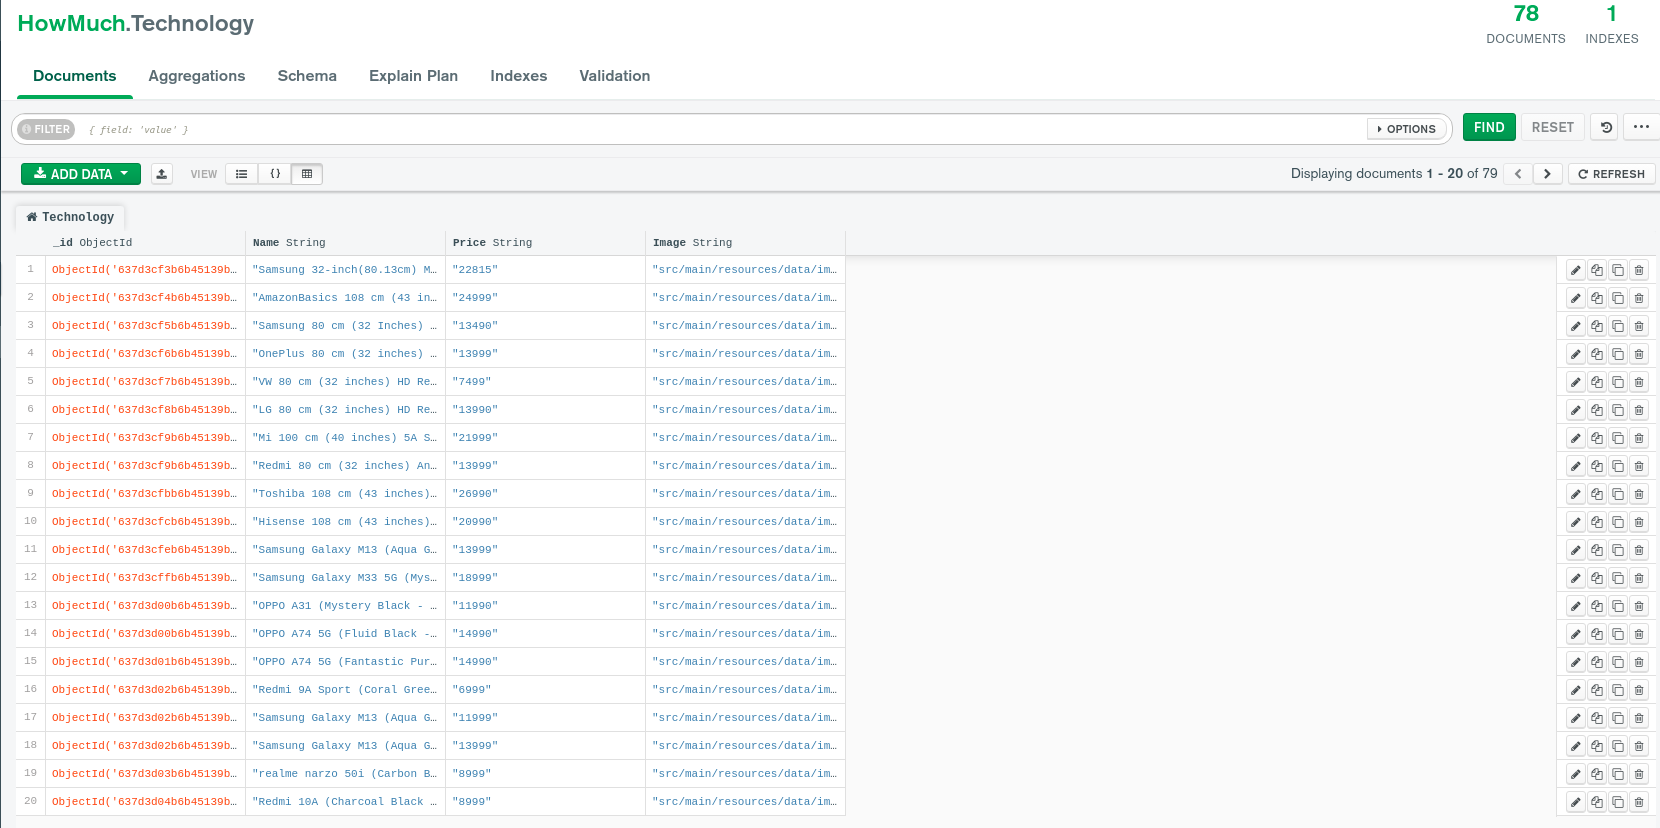
\includegraphics[scale=0.4]{mongo 1.png}
	\caption{A Screenshot of the MongoDB Compass Showing Records Stored in the Teachnology Schema}
\end{figure}

\begin{figure}[H]
	\centering
	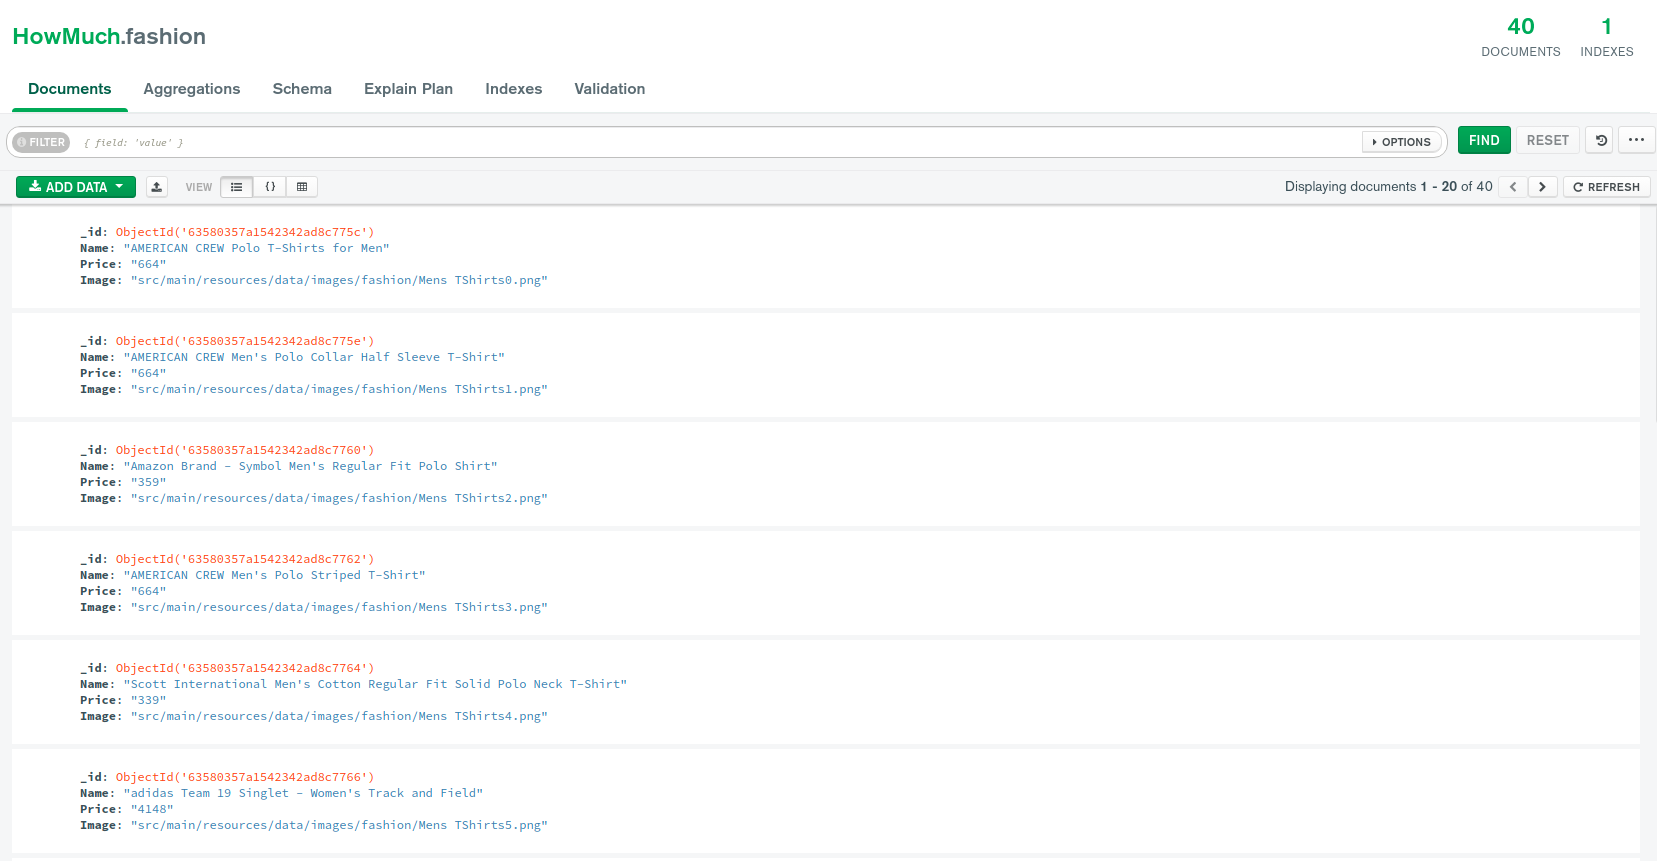
\includegraphics[scale=0.4]{mongo 2.png}
	\caption{Record Showing the Fashion Schema Documents}
\end{figure}
\subsection{Local CSV Files}
\begin{figure}[H]
\centering
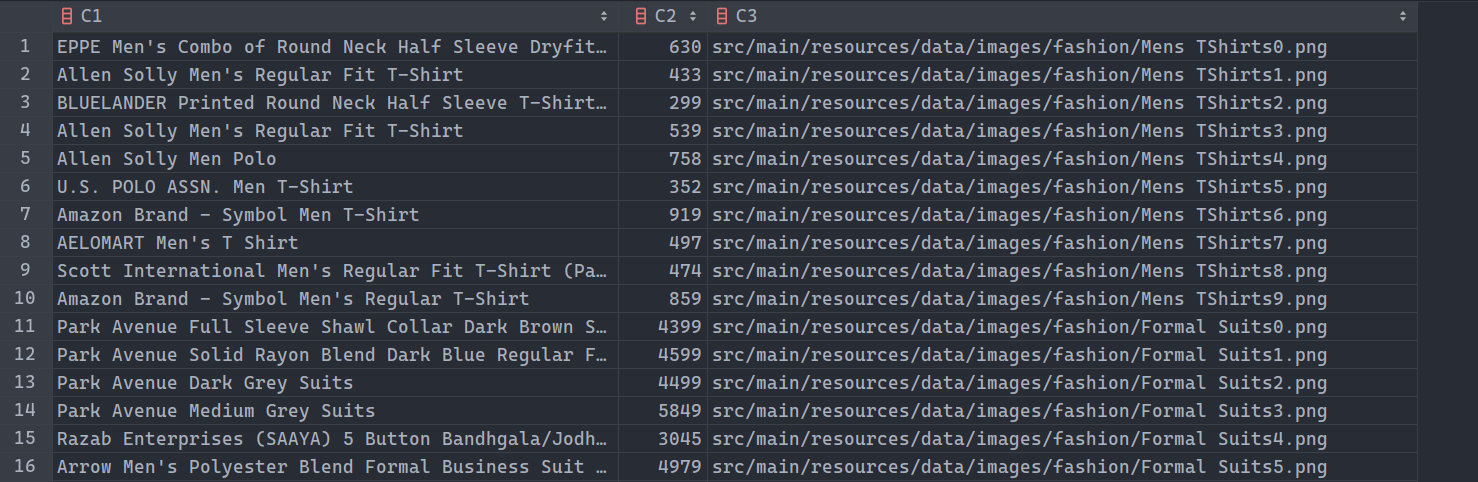
\includegraphics[scale=0.4]{csv.png}
\caption{Screenshot of the Local CSV File}
\end{figure}
\section{Unique Features}
\subsection{Dark Mode}
\subsection{Data Backup}
\subsection{Web Scrapping}
\subsection{Working Login and Account Creation}

\section{Screenshots of the Project}

\subsection{The Login Page}
\begin{figure}[H]
	\centering
	
\includegraphics[scale=0.45]{./design/Screenshots/Login Screen.png}
	\caption{The Login page after a successful login}
\end{figure}
\subsection{The Menu Screen}
\begin{figure}[H]
	\centering
	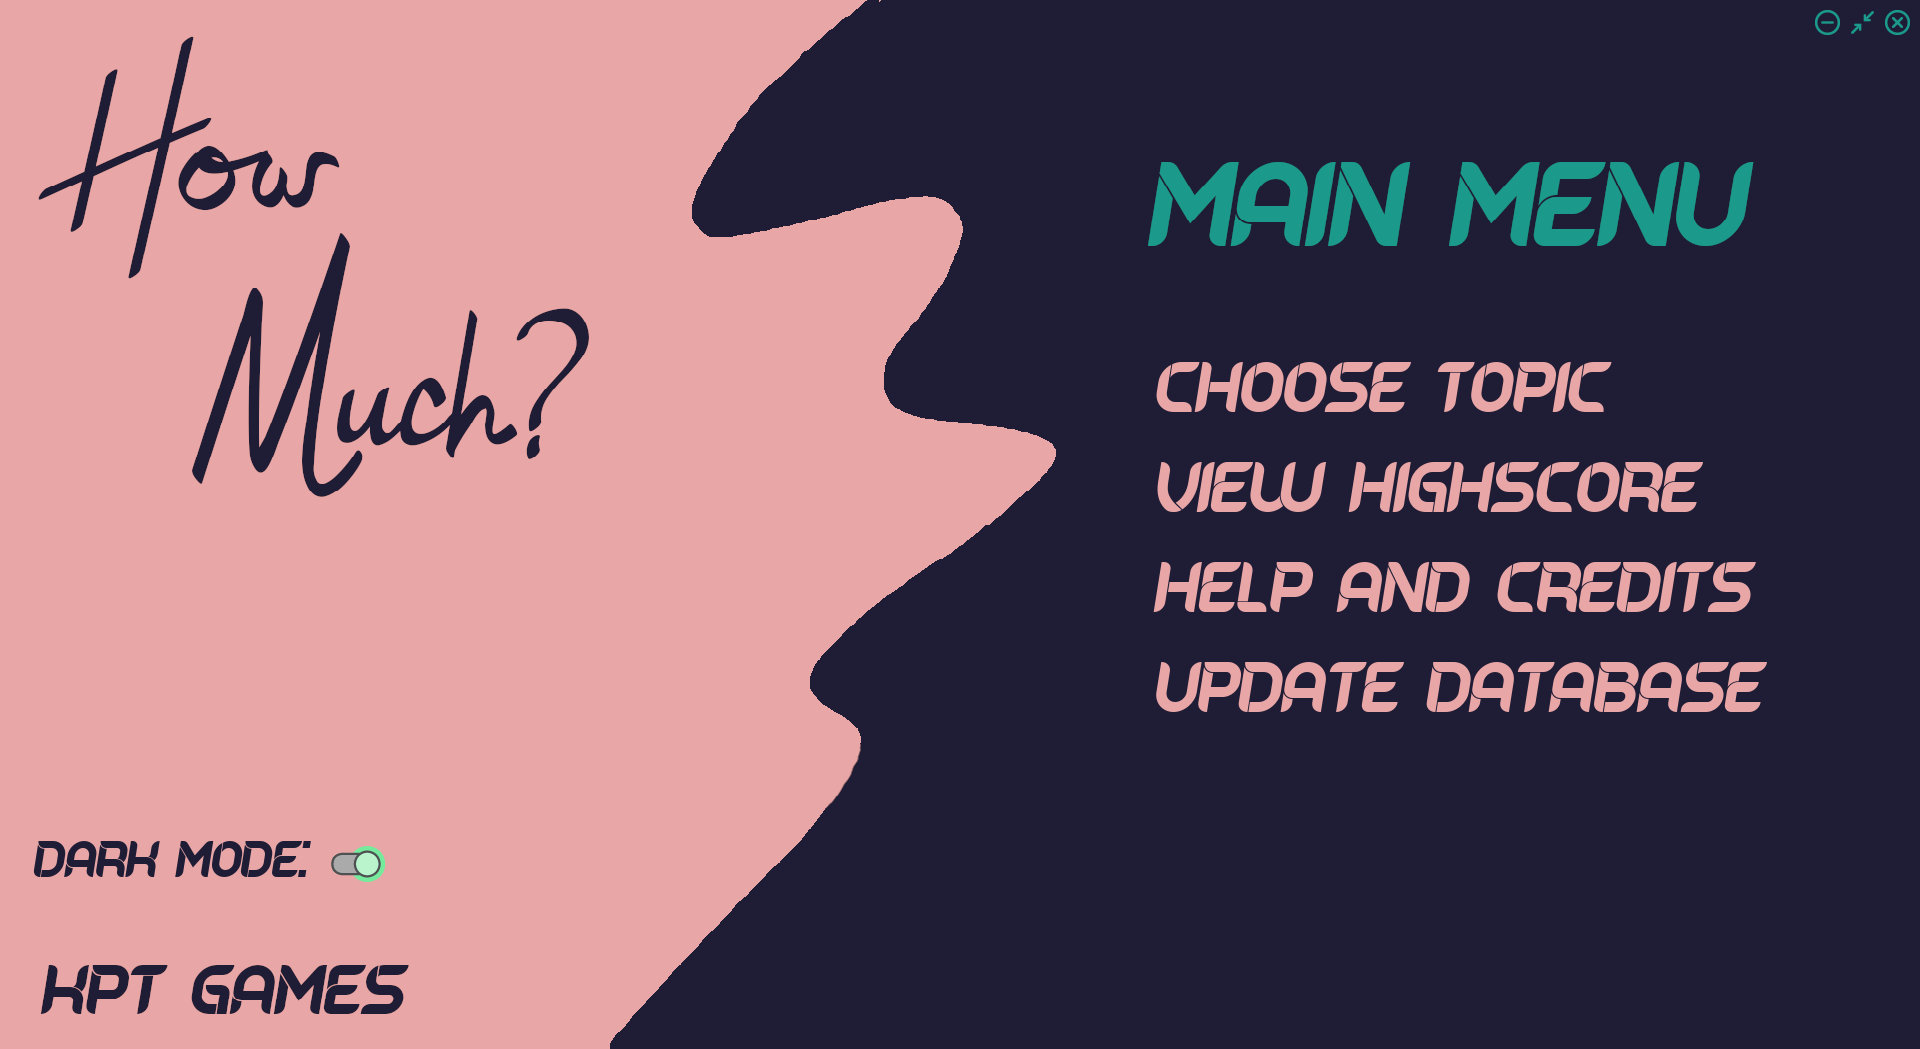
\includegraphics[scale=0.30]{./design/Screenshots/Main Menu Screen.png}
	\caption{}
\end{figure}


\subsection{The Topic Selection Screen}
\begin{figure}[H]
	\centering
	
\includegraphics[scale=0.30]{./design/Screenshots/Topic Selection.png}
	\caption{The Login page after a successful login}
\end{figure}
\subsection{The Highscore Screen}
\begin{figure}[H]
	\centering
	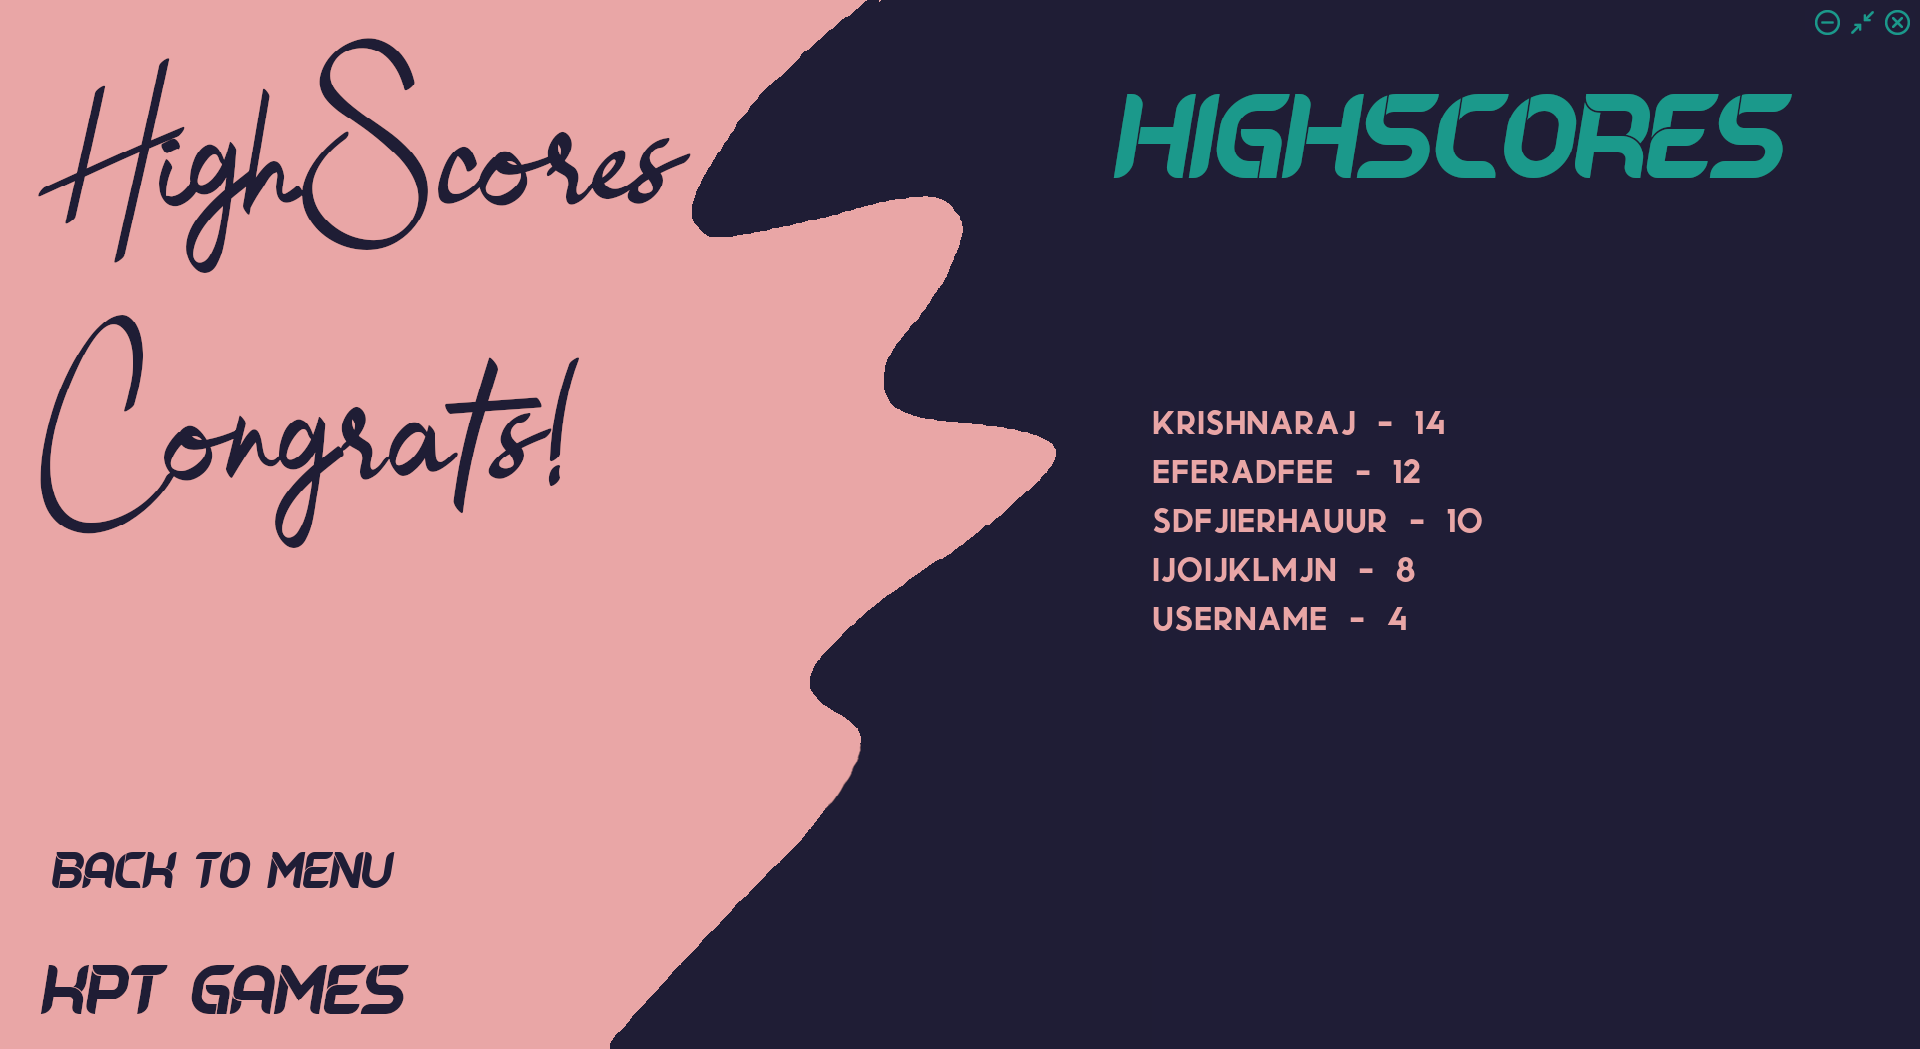
\includegraphics[scale=0.30]{./design/Screenshots/Highscores.png}
	\caption{The Login page after a successful login}
\end{figure}
\subsection{The Help and About}
\begin{figure}[H]
	\centering
	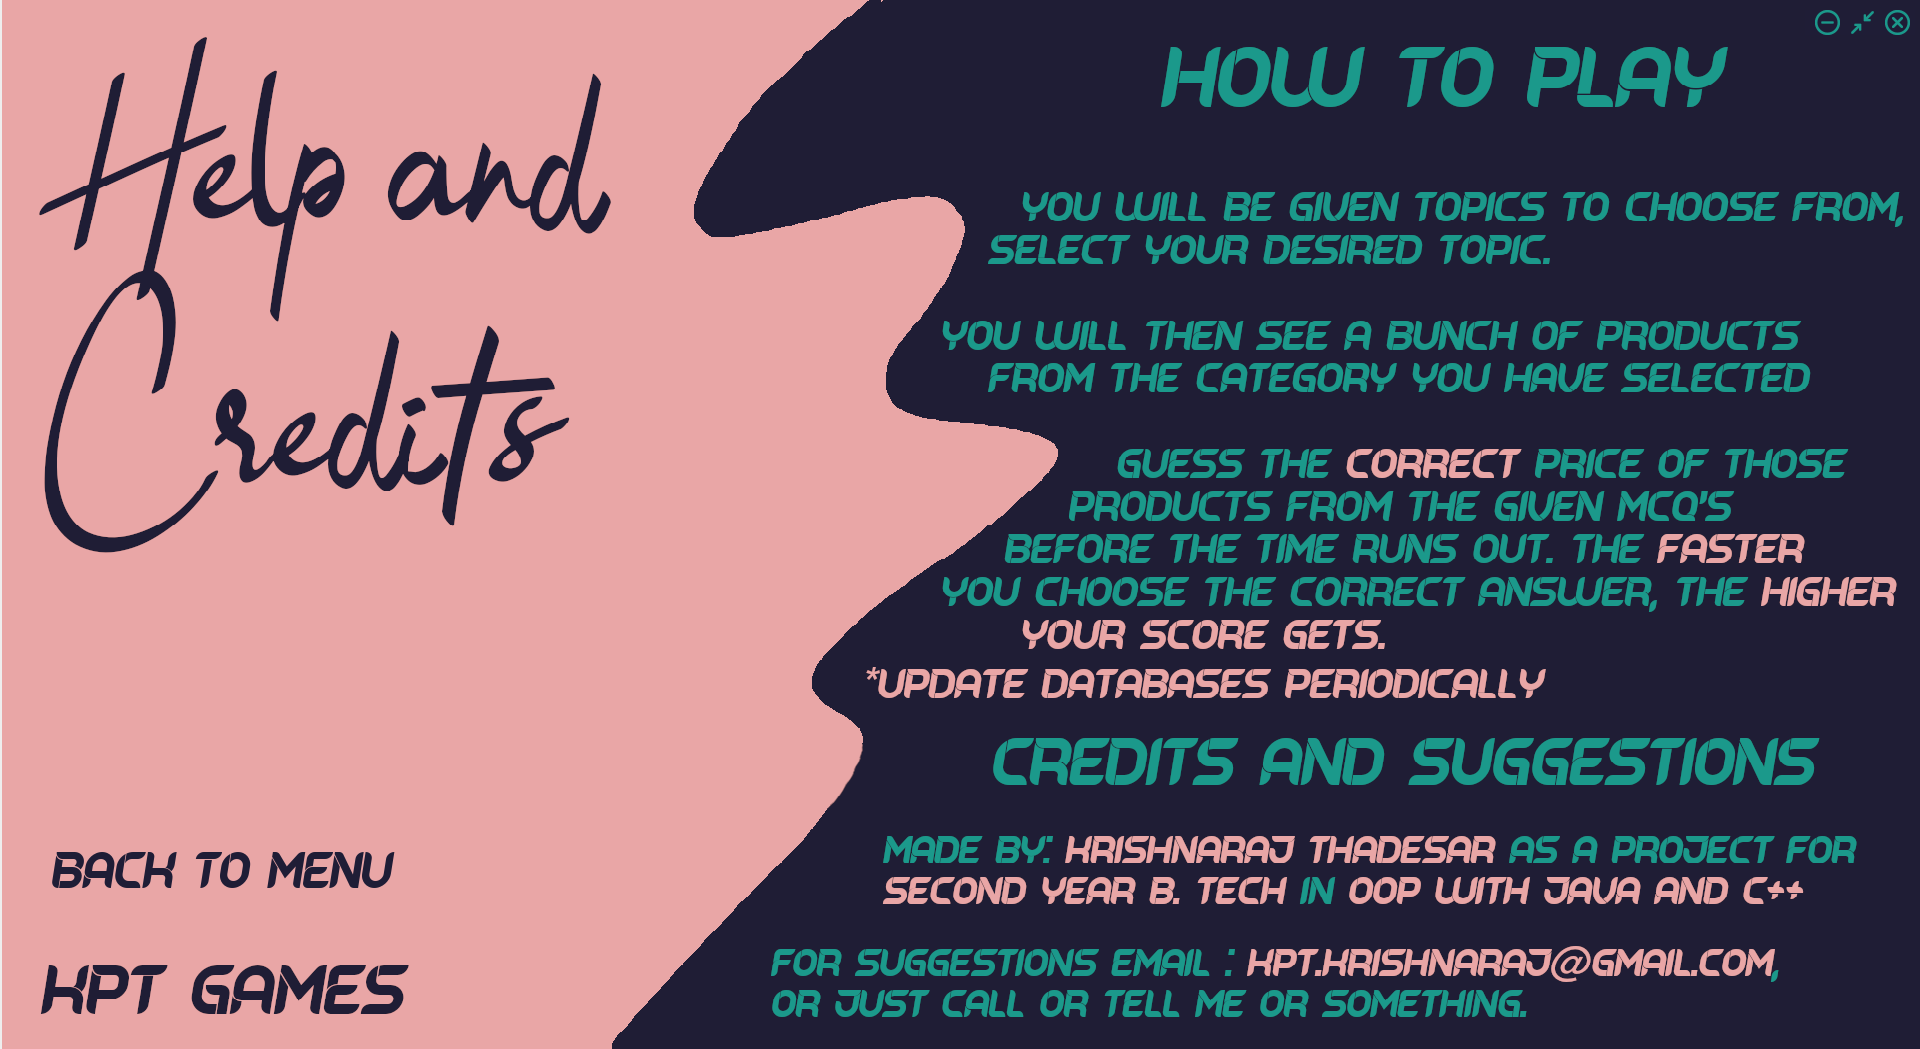
\includegraphics[scale=0.30]{./design/Screenshots/Help and Credits.png}
	\caption{The Login page after a successful login}
\end{figure}
\subsection{The Game Over Screen}
\begin{figure}[H]
	\centering
	
\includegraphics[scale=0.30]{./design/Screenshots/Game Over.png}
	\caption{The Login page after a successful login}
\end{figure}
\section{Output Files Produced}


\section{Walk-Through of the Files}

\subsection{Project Structure}
\begin{figure}[H]
	\centering
	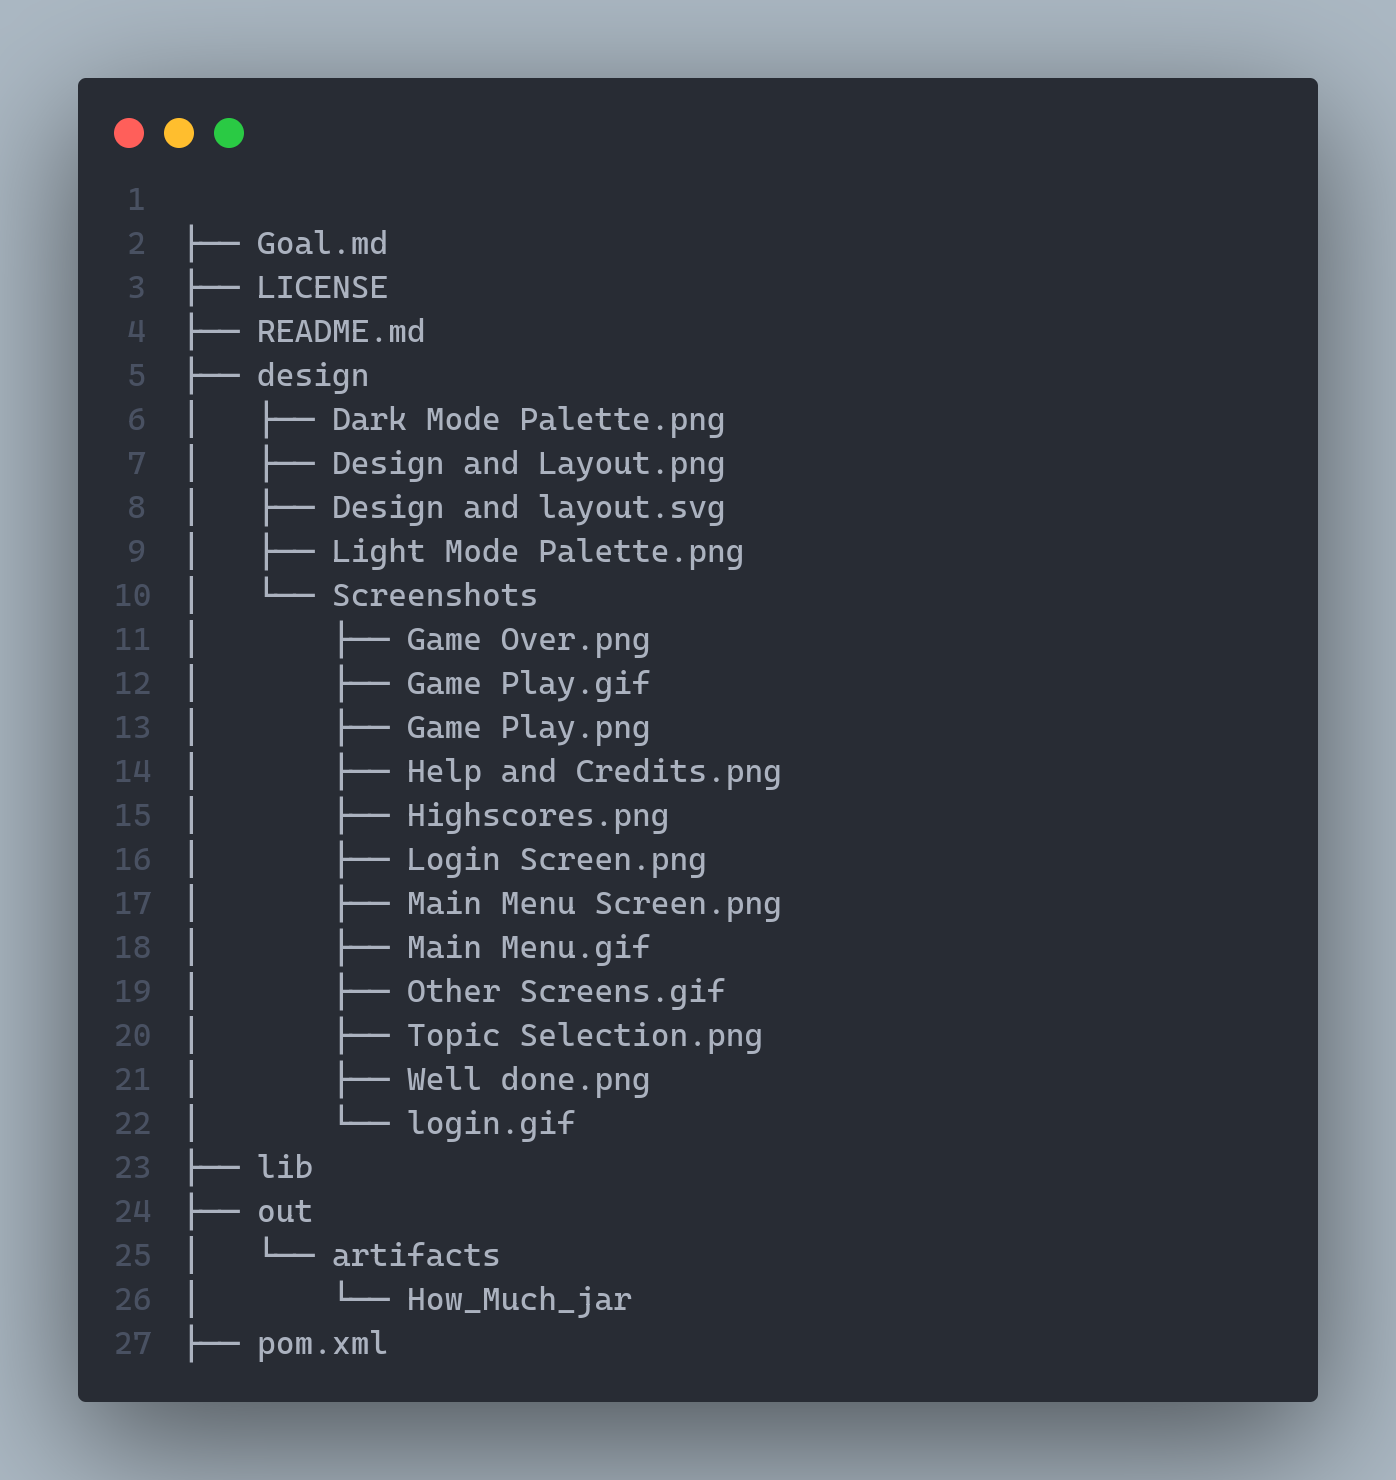
\includegraphics[scale=0.3]{code.png}
	\caption{}
\end{figure}
\begin{figure}[H]
	\centering
	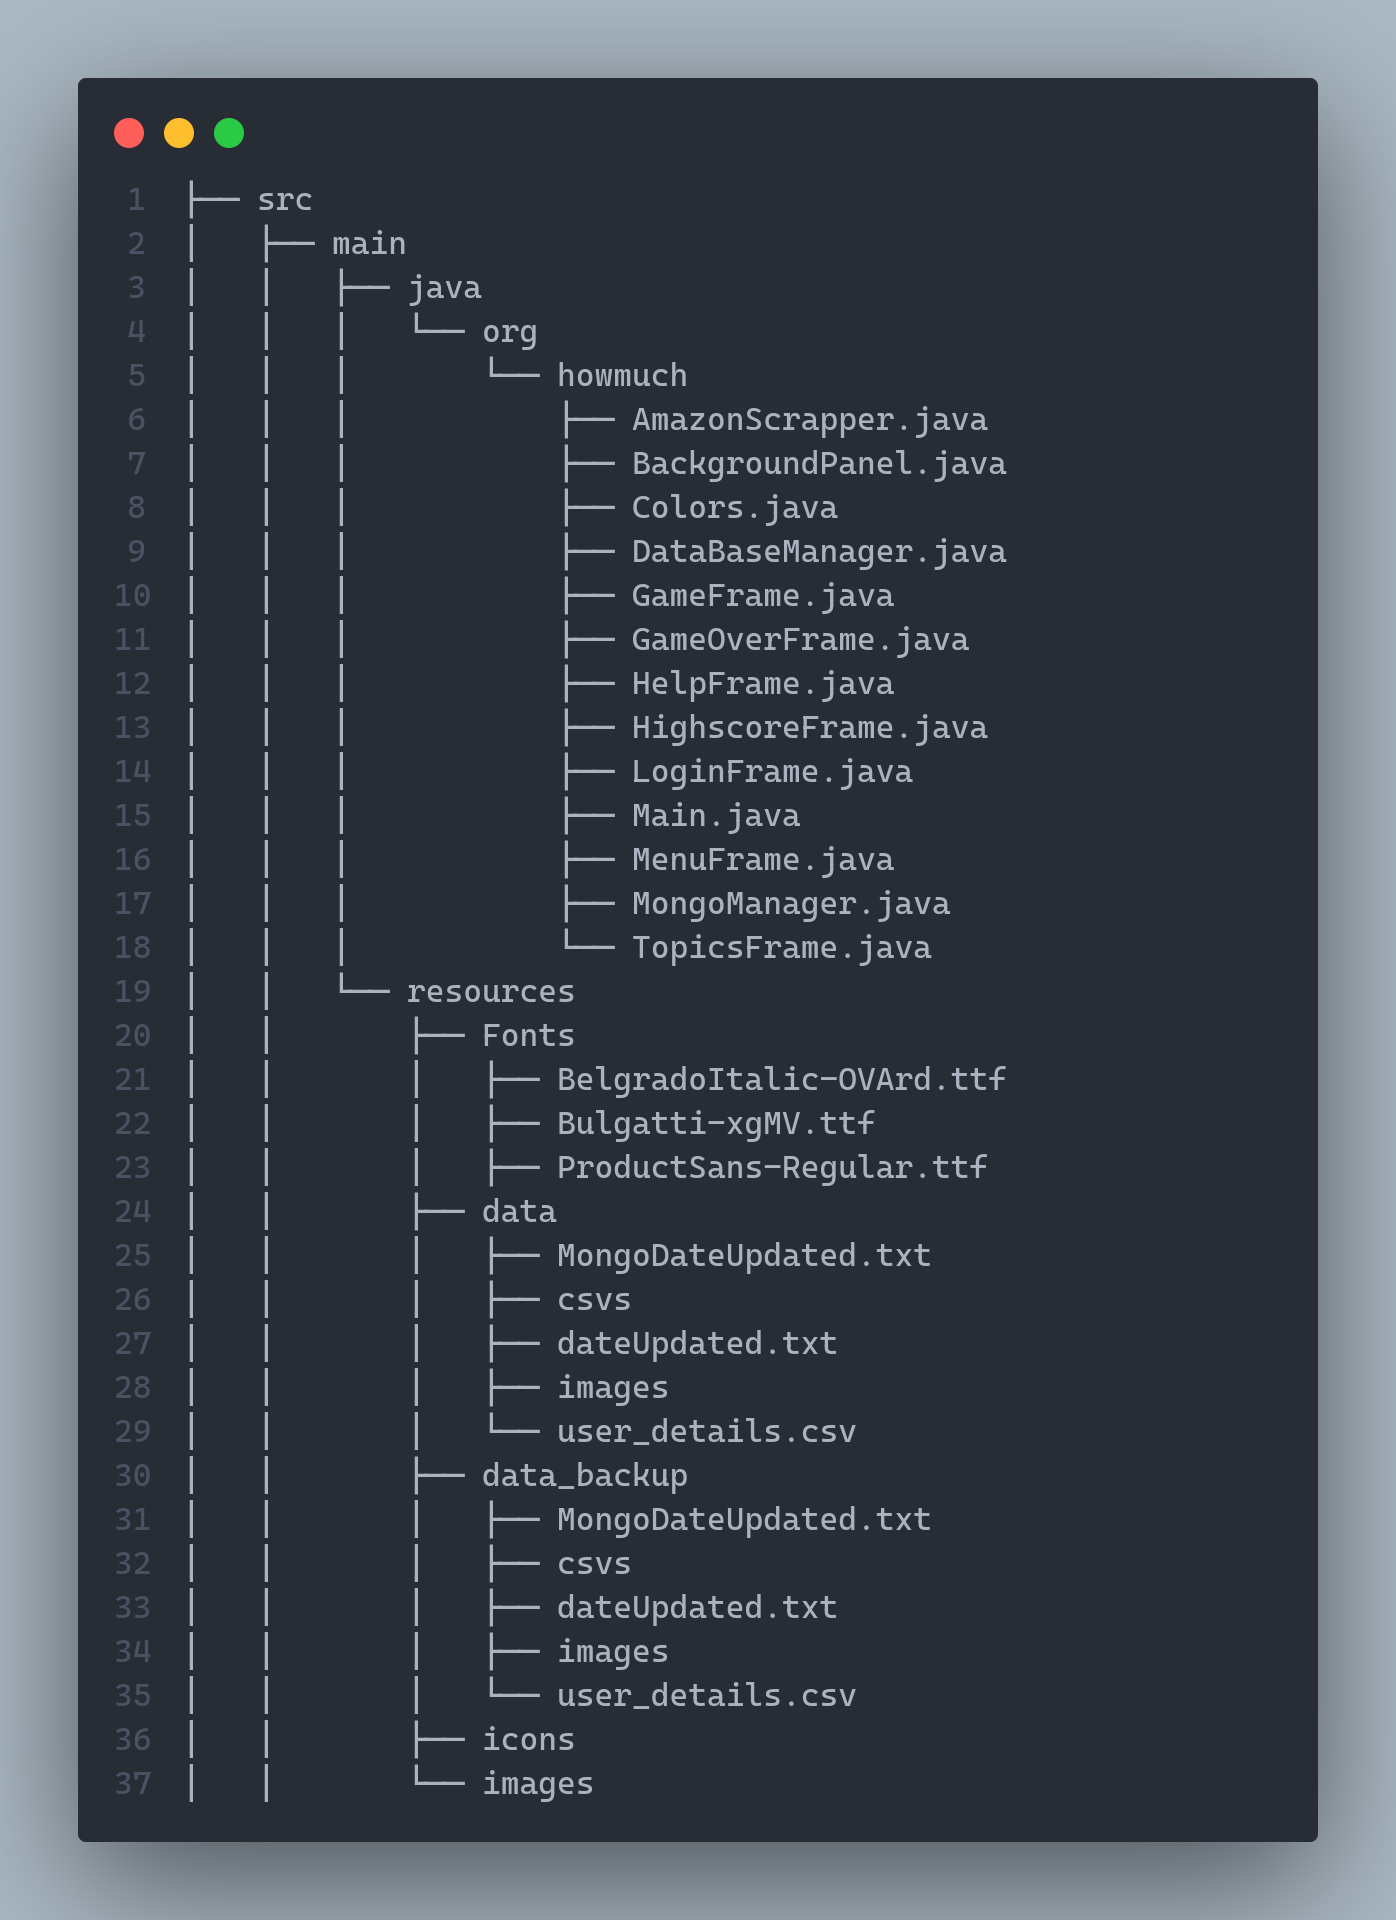
\includegraphics[scale=0.3]{code2.png}
	\caption{}
\end{figure}
\subsection{TopicsFrame.java}

\subsection{MongoManager.java}

\subsection{MenuFrame.java}

\subsection{Main.java}

\subsection{LoginFrame.java}

\subsection{HighscoreFrame.java}

\subsection{HelpFrame.java}

\subsection{GameOverFrame.java}

\subsection{GameFrame.java}

\subsection{  DataBaseManager.java}

\subsection{  Colors.java}

\subsection{  BackgroundPanel.java}

\subsection{  AmazonScrapper.java}

\section{Conclusion and Topics Learnt}

\section{Code File Main.java}

\lstinputlisting[language=Java, caption=Main Java file]{/run/media/krishnaraj/Programs/Java/How Much/src/main/java/org/howmuch/Main.java}



\end{document}